\documentclass[prb,aps,nobibnotes,twocolumn,doublespace,twocolumngrid,superbib]{revtex4}
%\documentclass[prb,aps,nobibnotes,superbib,preprint]{revtex4}

\usepackage{graphicx}
\usepackage{amsfonts}
\usepackage{amsmath}
\usepackage{bm}
\usepackage{alltt}
\usepackage{dcolumn} 
\usepackage{graphicx}
\makeatletter 
\makeatother

\begin{document}

\title{Linear scaling computation of the Fock matrix VIII. \\
       Periodic Boundary Conditions for Exact Exchange}

\author{C. J. Tymczak}
\author{Valery Weber}
\author{Eric Schwegler}
\author{Matt Challacombe}

\affiliation{Theoretical Division, Los Alamos National Laboratory, Los Alamos,
New Mexico 87545 }

\date{\today}

\begin{abstract}
We report on a consistent derivation of the exchange matrix for periodic
systems at the Gamma point. Previous work has always included k-space integration 
within the calculation of the exchange matrix. However, in  these methods
we can show that the calculation of the exchange matrix becomes inconsistent as the
region of k-space shrinks. This leads to a non-translation-ally invariant exchange matrix,
which is of major concern. We illustrate this problem and then show how, by a set of
simple ideas and arguments, we can correct this problem.
%
\vskip 0.07 in
\noindent{\bf Keywords}: Self-consistent-field, Exact-exchange, Linear-scaling, Gaussian-orbital 
%
\end{abstract}

\pacs{???}

\maketitle

\footnotetext[1]{\tt tymczak@lanl.gov}
\footnotetext[2]{\tt vweber@lanl.gov}
\footnotetext[3]{\tt schwegler@llnl.gov}
\footnotetext[4]{\tt mchalla@lanl.gov}
\footnotetext[5]{Preprint LA-UR XX-XXXX}


\section{INTRODUCTION}
Many calculations of the electronic structure of condensed matter systems now make use
of the exact exchange interaction 
\cite{Pisani80,REvarestov83,MCausa88,JAlmlof94,RDovesi00}. 
Whereas this has been a very
important functional in the quantum chemistry community 
\cite{PLowdin55,py,ASzabo89}, 
until the advent of the hybrid functionals 
\cite{Gill92,Becke93,ABecke96,Adamo99}, 
this functional has had very little impact on the
condensed matter electronic structure community. Now because of the accuracy obtainable with
the hybrid functionals, it has become very desirable to include exact exchange into
existing condensed matter electronic structure algorithms. 
However, most of these calculations make use of ${\bf k}$-space integrations to 
deal with the periodicity of the system \cite{RDovesi00}. However, this is not an ideal situation 
for linear scaling algorithms, where we would like to remove the need for doing
${\bf k}$-space integrations altogether by increasing the system size. 
However, when Gamma point only is attempted for exact exchange, a 
significant problem arises. For the Gamma point, in the limit of large system size,
we do not recover the ${\bf k}$-space energy per particle number; we do not have the correct
limit as particle number increases.  
%

In the proceeding sections we will first briefly review the Hartree
Foch equations of motion. Next, we will illuminate the problem that exist
for the calculation of the exchange matrix in the limit of the Gamma point for
periodic systems. We then give a solution to this problem, and then we verify that
the exchange matrix is correct in the limit of large systems as compared to a large 
${\bf k}$-space calculation done with {\bf Crystal98}. 
And finally, we verify that the exchange matrix build is indeed linear scaling
for the dense diamond system.

\section{The Hartree Fock Equations}
Within the Hatree fock approcimation we define the total energy as \cite{Pisani80,RDovesi00}
\begin{equation}
E = Tr[{\bf P} \, {\bf F}]+ E_{nn}
\label{HFEnergy}
\end{equation}
where the Fockian is defined as,
\begin{equation}
{\bf F} = 2 {\bf T}+2 {\bf V}_{en}+{\bf J}_{ee}+{\bf K}_x
\label{Fockian}
\end{equation}

\begin{eqnarray}
{\bf T}      & : & \,{\rm kinectic \, energy \, matrix} \nonumber \\
{\bf V}_{en} & : & \,{\rm electron-nuclear \, coulomb \, matrix} \nonumber \\
{\bf J}_{ee} & : & \,{\rm electron-electron \, coulomb \, matrix} \nonumber \\
{\bf K}_{x}  & : & \,{\rm exchange \, matrix} \nonumber \\
{E}_{nn}  & : & \,{\rm nuclear-nuclear \, repulsion \, energy} \nonumber \\ 
\label{Defin}
\end{eqnarray}
We solve for the density matrix, ${\bf P}$, via the eigen-equation 
\begin{equation}
{\bf F} {\bf P} = \epsilon {\bf P}
\label{DenMat}
\end{equation}
and iterate on equation (\ref{Fockian}) until self-cosistancy is reached.

\section{The Exchange matrix}
The exchange matrix calculated withing a LCAO basis set, including $k$-space, 
is define as  \cite{Pisani80,RDovesi00}
\begin{equation}
K_{ab}=\sum _{\mathbf{hgn}\,\,cd} \int
{{\phi _{a}(\mathbf{r}) 
\phi _{c+{\bf h}}(\mathbf{r}) 
P_{cd}[{\mathbf{n}}]\, 
\phi _{b+{\bf n}}(\mathbf{r'})
\phi _{d+{\bf n}+{\bf g}} ( \mathbf{r'})} \over {|{\bf r}-{\bf r'}|}} 
\label{CryEq}
\end{equation}a
where {\bf h},{\bf g}, and {\bf n} are the sum over bravi lattice vectors and $a-d$ are
the atom center basis functions. 
Let us consider two case; First let us consider the Gamma point, then in this case
\begin{equation}
P_{cd}[{\mathbf{n}}] \rightarrow P_{cd}[{0}]\, \delta _{{\mathbf{n},0}}
\label{NoN}
\end{equation}
Which allows us to rewrite equation (\ref{CryEq}) as
\begin{equation}
K_{ab}=\sum _{\mathbf{hg}\,\,cd} \int
{{\phi _{a}(\mathbf{r}) 
\phi _{c+{\bf h}}(\mathbf{r}) 
P_{cd}[0]\, 
\phi _{b}(\mathbf{r'})
\phi _{d+{\bf g}} ( \mathbf{r'})} \over {|{\bf r}-{\bf r'}|}} 
\label{NoNKab}
\end{equation}
However this is still not correct. Consider  figure \ref{figure:ExchangeRegion} where we
are depicting the exchange interaction of atom $a$ with all its neighbors. Equation
(\ref{NoNKab}) is the exchange interaction of atom $a$ with the central cell (gray region) in
figure \ref{figure:ExchangeRegion}, however, this neglects the exchange interaction 
between neighboring cells. This leads to an exchange matrix which is  not translationally invariant.
We could fix this by summing over the infinite set of lattice vectors ${\bf n}$, 
and this leads to a translationally invariant exchange matrix, but these integrals do not converge. 
Referring to figure \ref{figure:ExchangeRegion} we can see a simple fix to this problem. When 
we calculate the exchange matrix elements for atom $a$, include exchanges only within region
defined by the volume centered about atom $a$ (the red box in figure \ref{figure:ExchangeRegion}).
This gives both a convergent exchange matrix, and also a  translationally invariant one.
We do this by defining  a Minimum Image Distance (MID) condition, which is similiar to what is done
in Molecular Dynamics for the force on an atom due to neighboring cells \cite{awindemuth95}, 

\begin{equation}
K_{ab}=\sum _{\mathbf{hg}\,\,cd} \int
{{\cal MID}[ 
{\phi _{a}(\mathbf{r}) 
\phi _{c+{\bf h}}(\mathbf{r}) 
P_{cd} \, 
\phi _{b}(\mathbf{r'})
\phi _{d+{\bf g}}( \mathbf{r'})]} \over {|{\bf r}-{\bf r'}|}} 
\label{MinImageKab}
\end{equation}
where $\cal MID$ is a function which shifts the distributions to there nearest image.
In pseudocode,
\begin{itemize}
\item[] {{\bf Input[}$\psi_a({\bf r})\psi_c({\bf r+R})$,$\psi_b({\bf r'})\psi_d({\bf r'+R'})${\bf ]}}
\item[] {{\hskip 0.2 in}${\bf D}\,\,\,\,={\bf AC} - {\bf BD} $}
\item[] {{\hskip 0.2 in}${\bf FD}=frac[{\bf D}$]}
\item[] {{\hskip 0.2 in}${\bf FD}={\bf FD}-aint[{\bf FD}]$}
\item[] {{\hskip 0.2 in}${\bf D}\,\,\,\,=atom[{\bf FD}]$}
\item[] {{\hskip 0.2 in}$I\,\,\,\,\,\,=(ac|bd)$  }
\item[] {{\bf Output[}$I${\bf ]}}
\end{itemize}
Which we have implimented into our integral code.

The problem with the ${\bf k}$-space convergence, which is extreme for the Gamma point, 
will also exist for any finite set of lattice vectors ${\bf n}$. Consider 
figure \ref{figure:ExchangeRegion_k111} where we show the regions that atom $a$ exchanges with
for a maximum ${\bf k}$-space of ${\bf k}_{max} = \{1,1,1\}$. Here we see again that the integral
defined in equation (\ref{CryEq}) is over the wrong region for atom $a$, and can be easily 
rectified by the MID condition. As can also be easily seen this problem will disappear as the 
region of ${\bf k}$-space increases because of the exponential decay of the density matrix with 
distance.

\section{Verification}

Table \ref{table:ComToCrystal98} shows our results for the total
energy for Magnesium Oxide as compared to results obtained from \textbf{Crystal98}.
for the STO-3G basis set for increasing system size. We see that we obtain excellent
convergence to the {\bf Crystal98} large ${\bf k}$-space calculation. This verifies that
our methodology for doing the exchange matrix at the Gamma point is correct, and converges 
in the correct fashion in regard to increasing system size.

\section{Scaling}
 
Figure \ref{figure:Scaling_Matrix_Build} the time it takes to build the
matrix  \( K_{x} \) for the dense diamond periodic system up to 800 atoms for the
basis set 6-31G$ ^\dagger$ \cite{Pople92} at a {\it loose} level of accuracy.
Also included in the figure for comparision are the total time for the
density matrix solver, TRS4 \cite{ANiklasson03}, 
and the Coulomb matrix build using our Quantum chemical treee code \cite{CTymczak03c}. 


%We also show in figure \ref{figure:EnergyPerN} the energy per carbon atom and 
%in figure \ref{figure:ErrorPerN} the relative error in the total energy. 
%Again we see the convergence of the total energy
%as a function of increasing system size, which is akin to k-space integration.
%We also see that our relative error is very well controlled within the \
%textbf{MondoSCF} quantum chemistry code, even up to 512 carbon atoms.


\section{CONCLUSIONS}
We have shown a consistent derivation for the exact exchange integrals at the $\Gamma$-point. 

\section*{ACKNOWLEDGMENTS}

We would like to acknowledge Tommy Sewell and Ed Kober for there advise
and support. We would also like to thank Anders Niklasson for his help
in preparation of this manuscript. 

\bibliographystyle{apsrmp} 
\bibliography{mondo_new} 


\eject

\begin{table}
\caption{Comparison \textbf{MondoSCF} and \textbf{Crystal98} for a 
Magnesium Oxide test system within the Hartree-Fock approxiamtion using
the STO-3G basis set. The \textbf{MondoSCF} calculations where done to
the accuracy of the quoted digits. All calculations where done at the Gamma point
for comparison except the last \textbf{Crystal98} calculation, which was done at 
${\bf k}_{max}=\{6,6,6\}$.}
\label{table:ComToCrystal98}
\center{
\begin{tabular}{lcll}
\toprule
{\sc MondoSCF}  & 8$^g$    & -1098.4382  & -137.30478 \\
                & 16$^f$   & -2197.0564  & -137.31603 \\
                & 32$^g$   & -4394.4846  & -137.32764 \\
                & 54$^f$   & -7415.8962  & -137.33141  \\
                & 64$^g$   & -8789.2494  & -137.33202  \\
                & 128$^f$  & -17578.502  & -137.33205 \\
                & 216$^g$  & -29663.729  & -137.33208 \\ 
\hline
${\sc Crystal98}^h$  & 32$^g$   & -4394.5847  & -137.33077 \\
                     & 64$^g$   & -8789.2484  & -137.33201 \\
\hline
${\sc Crystal98}^i$  & 2$^f$    & -274.66415  & -137.33208  \\ 
\botrule
$ ^f$Triclinic \\
$ ^g$Cubic  \\
\multicolumn{4}{l}{$ ^h$Gamma Point.} \\
\multicolumn{4}{l}{$ ^i8\times8\times8$ $k$-space grid.}
\end{tabular}}
\end{table}

\begin{figure}
\caption{Unit cell and its brava lattice vectors.}
\label{figure:SimCell}
{\centering \includegraphics{UnitCell_2.ps} \par}
\end{figure}
%
%
%
\begin{figure}
\caption{For the Gamma point, the region in which atom $a$ has exchange interactions.}
\label{figure:ExchangeRegion}
{\centering \includegraphics{ExchangeRegion.ps} \par}
\end{figure}
%
%
%
\begin{figure}
\caption{For ${\bf k}_{max}=\{1,1,1\}$, the region in which atom $a$ has exchange interactions.}
\label{figure:ExchangeRegion_k111}
{\centering \includegraphics{ExchangeRegion_k111.ps} \par}
\end{figure}
%
%
%
\begin{figure}
\caption{Scaling results for the exchange matrix build, the coulomb matrix
build (scaled by ten), and the density matrix solver (scaled by twenty),  
for the dense diamond periodic system up to 800 atoms using the
6-31G$ ^\dagger$ basis set.}
\label{figure:Scaling_Matrix_Build}
{\centering \includegraphics{Timing_Diamond_ONX.ps} \par} 
\end{figure}
%
%
%
\begin{figure}
\caption{Energy per Carbon atoms vs. Lattice constants for an 8 atom 
unit cell with the 6-31G$ ^\dagger$/HF basis set and a tight level of accuracy. Also
shown is the same calculation, but in a 216 atom unit cell at a losse level
of accuracy.}
\label{figure:EnergyVsLattice}
{\centering \includegraphics{Timing_Diamond_ONX.ps} \par} 
\end{figure}

%
%
%
%\begin{figure}
%\caption{ Energy per carbon atom for the dense diamond
%periodic system up to 512 atoms using the {\bf Crystal98} basis set 6-21G* \cite{CBS:621G:C}.}
%\label{figure:EnergyPerN}
%{\centering \includegraphics{blank.ps} \par} 
%\end{figure}
%
%
%
%\begin{figure}
%\caption{ Relative Error per carbon atom for the dense diamond
%periodic system up to 512 atoms using the {\bf Crystal98} basis set 6-21G* \cite{CBS:621G:C}.}
%\label{figure:ErrorPerN}
%{\centering \includegraphics{blank.ps} \par} 
%\end{figure}



\end{document}
